\chapter{Introdução}
\label{chap:intro}
O Brasil apresenta uma matriz energética diferente da do resto do mundo, onde as fontes renováveis representam uma grande parte da geração da energia. Segundo a \cite{epe_site}, em 2016, a matriz energética mundial contava com somente 14,1\% da matriz energética constituída por fontes renováveis, enquanto o brasil já apresentava 82\% da sua matriz vinda de fontes renováveis, onde a geração hidrelétrica corresponde a 70\% dessa geração.

A expectativa é de que a energia hidrelétrica continue sendo cada vez mais utilizada no país, devido ao crescimento previsto da demanda energética brasileira, onde segundo o \cite{atlas_aneel} o consumo atual é de 405 TWh e a demanda esperada em 2030 é de 950 e 1.250 TWh/ano \cite{bronzatti_matrizes}. Mesmo com a grande participação da geração hidrelétrica , somente 23\% dos 260 GW totais de potencial hidrelétrico são aproveitados \cite{atlas_aneel}.

A concentração de demanda energética no Brasil está concentrada principalmente na região Sudeste devido a densidade populacional e elevada industrialização, isso faz com que dois terços do total da  capacidade instalada estejam localizadas na Bacia do Rio Paraná  que é a bacia mais pŕoxima da região, enquanto as bacias com potencial menos aproveitado são as localizadas no norte e nordeste do país \cite{atlas_aneel}.

Com desenvolvimento do país é esperado um aumento na demanda de energia elétrica e consequentemente um aumento na geração de energia hidrelétrica, isso faz com que seja esperado um crescimento considerável na quantidade das linhas de transmissão, de acordo com \cite{MME}, em setembro de 2018 o sistema elétrico brasileiro já atingiu 144.828 km de linhas de transmissão.  Esse aumento na quantidade de linhas tende a ser amplificado pela tendência à exploração da geração de energia na região Norte, assim sendo necessário a construção de novas linhas para distribuir essa energia para as outras partes do País.

Quanto mais linhas de transmissão e maiores distâncias entre os centros geradores, maiores tendem a ser as perdas. Isso faz com que seja necessária um controle da qualidade dessa transmissão, o que se dá por meio de inspeções. A estrutura já existente apresenta precariedade em alguns aspectos, onde segundo \cite{rangel2009sistema} “no Brasil, há uma quantidade considerável de linhas de transmissão que já ultrapassou os 40 anos de idade. Com o envelhecimento das linhas de transmissão, a manutenção preventiva é um fator de extrema relevância para garantir o perfeito funcionamento dos sistemas.”
A necessidade da constante manutenção e a alta periculosidade que os operadores são expostos faz com novas alternativas e tecnologias sejam aplicadas para a manutenção, o uso de Drones pilotados remotamente, com câmeras e sensores já é uma realidade em alguns países do mundo. O desenvolvimento de um robô próprio para inspeção de linha configura uma dessas novas alternativas, e possibilita uma expansão dos horizontes para as tecnologias aplicadas.
%--------- NEW SECTION ----------------------
\section{Objetivos}
\label{sec:obj}
O objetivo do trabalho é implementar o sistema de movimentação do robô ELIR (\textit{Electrical Line Inspection Robot}). Onde esse sistema é complementar aos outros existentes no robô, onde o conjunto dessas soluções busca fundamentar a implementação de uma Inspeção autônoma da linha.


\subsection{Objetivos Específicos}
\label{ssec:objesp}
Para o desenvolvimento do sistema é necessário realizar o estudo da movimentação, gestão de energia, controle e elaboração de trajetória para sistemas robóticos. A operação na linha faz com que seja necessário a gestão de energia do robô, assim como a integração com os outros subsistemas já desenvolvidos. De forma a garantir a operação na linha, os dispositivos e ferramentas utilizadas devem estar integradas no ROS (\textit{Robot Operating System}), onde é necessário também a integração com outros pacotes já desenvolvidos para o Robô.

%--------- NEW SECTION ----------------------
\section{Justificativa}
\label{sec:justi}
 Tendo em vista a crescente demanda de energia elétrica do país bem como a previsão , a necessidade de um processo confiável de transmissão se torna amplamente necessário, afinal, diversas unidades consumidoras são alimentadas diariamente, além de instalações que exercem atividades críticas, como hospitais. As unidades geradoras de energia elétrica se encontram em regiões distantes de seus consumidores finais, portanto se faz necessário a utilização de linhas de transmissão de energia elétrica. 
 
 Uma linha de transmissão é uma linha composta por cabos condutores de energia elétrica, utilizada para a transmissão de energia em alta tensão, saindo da origem geradora e indo até às cargas consumidoras.
 
 A garantia da distribuição em condições favoráveis se dá pela confiabilidade das linhas de transmissão e os procedimentos de manutenção aplicados à elas, para isso, é realizada constantemente a rotina de inspeção nas linhas. A rotina de inspeção, se dá através da análise da integridade da estrutura das torres, a condição em que se encontram os isoladoras e as conexões das linhas de transmissão, uma vez que o tempo e a exposição a umidade e ao sol, além de diversos eventos climáticos, fazem com diversas falhas referentes ao desgaste do material venham a aparecer. 
 
 Estas análises têm como principal objetivo a detecção de eventuais pontos de ruptura. Outro meio para a localização dos eventuais pontos de ruptura se dá pelo uso de câmeras térmicas, onde existe o aumento da temperatura pontual devido à elevação na resistência elétrica. 
 
 \begin{figure}[h!]												
 	\centering												
 	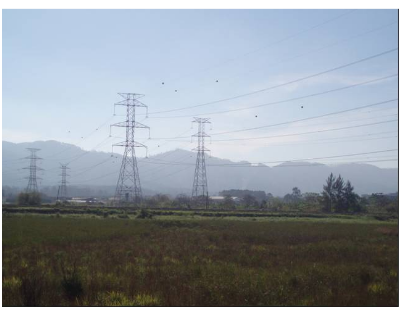
\includegraphics[width=0.5\textwidth]{Estrutura_linha.png}			
 	\caption{Instalação típica de uma linha de transmissão}		
 	\label{img:Estrutura_Linha}	
 	\source{\cite{rangel2009sistema}}		
 \end{figure}
 
 Segundo \cite{rangel2009sistema}, as rotinas de inspeção de linhas de transmissão se dão principalmente por dois métodos: inspeções por aeronaves e inspeções terrestres.
 A inspeção realizada por aeronaves, se dá tipicamente com o uso de helicópteros, que executam voos em baixa altitude, extremamente próximos das linhas de transmissão. 
 
 Em alguns casos as condições climáticas podem dificultar o procedimento de inspeção e controle da aeronave, além do risco inerente da atividade para os tripulantes, principalmente devido ao fato de que as aeronaves tipicamente operam na região de “homem-morto”, uma zona de altura que representa perigo para os operadores a bordo das aeronaves.
 
  \begin{figure}[h!]												
  	\centering												
  	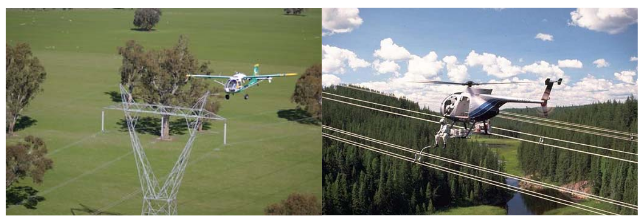
\includegraphics[width=0.5\textwidth]{Inspecao_metodos.png}			
  	\caption{Inspeção em linhas de transmissão por veículos aéreos tripulados.}		
  	\label{img:Inspecao_metodos}	
  	\source{\cite{rangel2009sistema}}		
  \end{figure}
 
 A inspeção por vias terrestres possui uma grande dificuldade devido à dependência do terreno do local, o qual pode ser de difícil acesso devido às características geográficas.Diversos fatores tornam a inspeção de linhas de transmissão um procedimento não só perigoso, mas também altamente custoso. 
 
 Segundo \cite{cinematicajuliana} as principais desvantagens dos meios convencionais de inspeção de linhas de transmissão são os riscos de acidentes, devido a periculosidade do procedimento de inspeção; o alto custo, uma vez que é necessário a locação e deslocamento de equipamentos específicos para o transporte e inspeção das linhas de transmissão; a alta dependência das condições climáticas e geográficas, uma vez que se torna muito difícil realizar rotinas de inspeção em tempos chuvosos ou em locais de difícil acesso.
 
 Outra grande desvantagem dos procedimentos de inspeção definida por \cite{cinematicajuliana} é justamente a necessidade de uma mão de obra qualificada para realização destes procedimentos. Se estes procedimentos de inspeção de linha de transmissão fossem realizados em linhas desenergizadas, o processo seria bem mais simples e rápido, porém existem diversos problemas atrelados ao fato de que existem inúmeras cargas consumidoras que necessitam da energia elétrica gerada.


%--------- NEW SECTION ----------------------
\section{Organização do \thetypework}
\label{section:organizacao}
O documento está organizado em cinco capítulos, seguindo a seguinte estrutura:

\textbf{Capitulo 1 - Introdução}: Faz a contextualização do âmbito no qual a pesquisa proposta
está inserida. Apresenta, portanto, a problemática, objetivos e como este projeto Theoprax de conclusão de curso está estruturado


\textbf{Capítulo 2 - Referencial Teórico}: Apresenta a base teórica necessária para o desenvolvimento do projeto.

\textbf{Capítulo 3 - Metodologia}: Define o método adotado para o desenvolvimento do projeto, explicitando seu fluxo de atividades e entradas fornecidas pelo cliente.

\textbf{Capítulo 4 - Desenvolvimento e testes}: Exibe os resultados obtidos durante o desenvolvimento do
projeto, apresentando-os em testes unitários e integrados, assim como as datas de quando foram realizado, e os responsáveis pela execução.

\textbf{Capítulo 5 - Conclusão}: Apresenta as conclusões, contribuições e algumas sugestões de atividades de pesquisa a serem desenvolvidas futuramente.

